\chapter{Praktická aplikace}
Vzhled a ovládání celé aplikace je velmi jednoduché a intuitivní. Na úvodní stránce je přehled všech zařízení zapojených do sítě včetně jejich stavu. Vedle názvu zařízení je vidět, jestli je online, či nikoliv. Pod názvem je vidět aktuální přijatá informace v číselné podobě. Následuje seznam připojených a připojitelných zařízení. Jedním kliknutím je možné propojit jakékoliv koncentrátory. V tu chvíli začne server přeposílat příchozí data na všechna připojená zařízení. Počet připojitelných zařízení není nijak omezen. Toto je velká výhoda celého projektu. Není totiž vázán na fyzická spojení a příchozí data je tak možné poslat všem v síti bez dalších technických komplikací.

\begin{figure}[h]
    \centering
	\makebox[\textwidth]{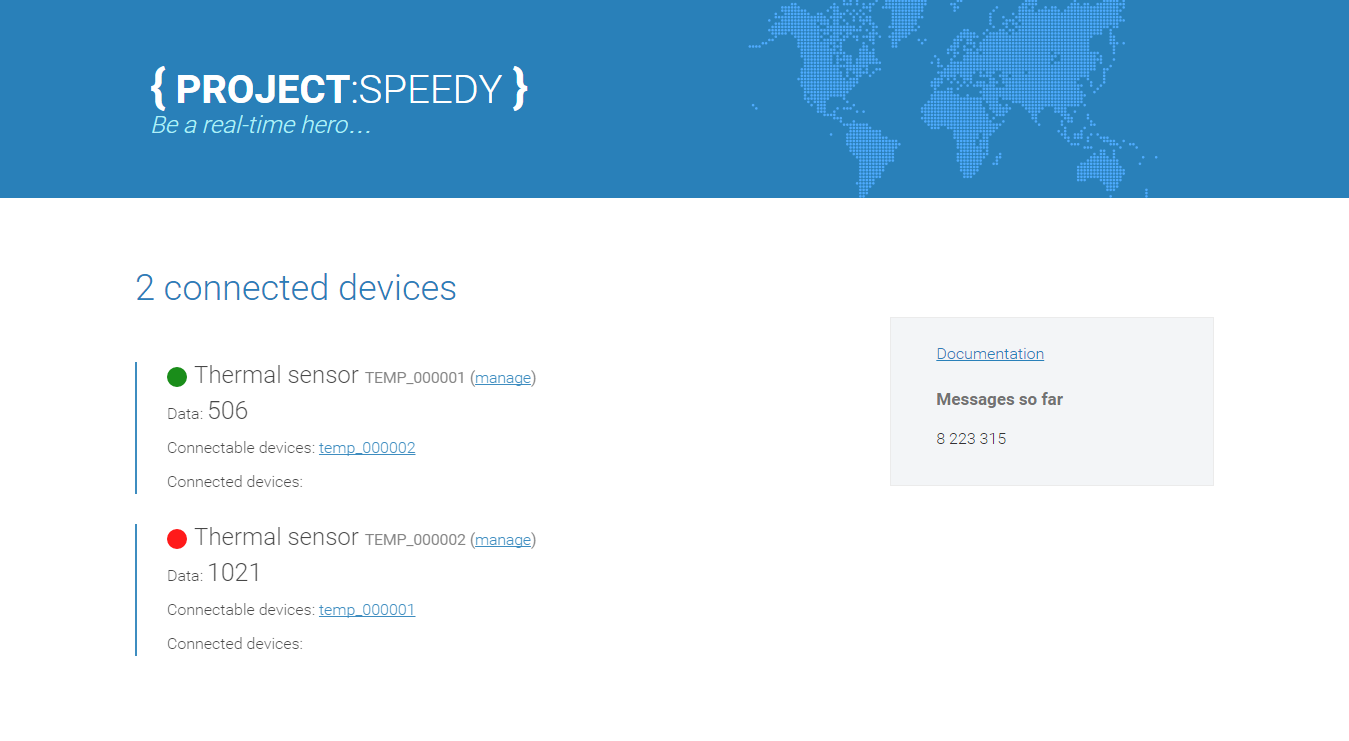
\includegraphics[width=\textwidth]{img/speedy1.png}}
	\caption{Úvodní stránka aplikace - přehled připojených zařízení}
	\label{fig:speedy1}
\end{figure}

Detail konkrétního zařízení poskytuje podobný pohled, navíc však ukazuje dodatečné informace jako jsou například IP adresy, nebo čas posledního ohlášení. Kromě samotné vizualizace historie příchozích dat je možné nastavit charakter dat odchozích. To znamená, že když bude připojeno další zařízení, nebudou se data rovnou přeposílat, ale najde se příslušná hodnota podle zvolené funkce a tato hodnota se pošle. Ve výchozím stavu se vše chová lineárně, tzn. jaká informace přijde, taková se přeposílá. Je však možné zvolit exponenciální viz rovnice \ref{eq:exp}, logaritmický \ref{eq:log}, nebo vlnitý charakter \ref{eq:vlna}. Poslední variantou je boolean závislost, kdy do hodnoty 512 včetně je výstupem 0, jinak maximální hodnota.

\begin{equation}
	y_{\_exp} = 1.80753 \cdot 1.00625^x
	\label{eq:exp}
\end{equation}

\begin{equation}
	y_{\_log} = -1053.96 + 289.931 \cdot ln(x)
	\label{eq:log}
\end{equation}

\begin{multline}
	y_{\_vlna} = -3.23206 \cdot 10^{-8} \cdot x^4 + 0.000068 \cdot x^3 - 0.044362 \cdot x^2 + \\
				+9.59513 \cdot x - 47.9076
	\label{eq:vlna}
\end{multline}

\begin{figure}[H]
	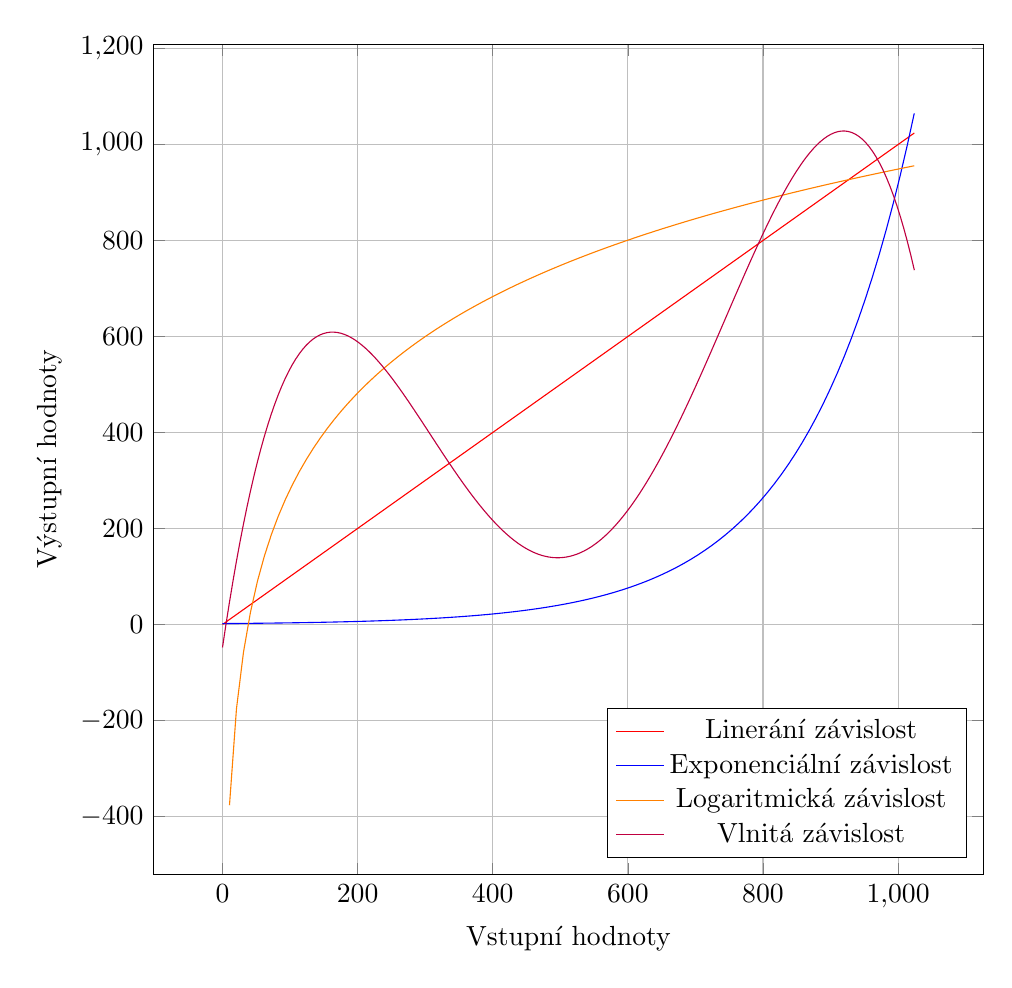
\begin{tikzpicture}
		\begin{axis}[width=1\textwidth,height=1\textwidth,xlabel={Vstupní hodnoty},ylabel={Výstupní hodnoty},legend style={at={(0.98,0.11)},anchor=east},grid=major]
			\addplot[red,domain=0:1024,samples=10]{x};
			\addlegendentry{Linerání závislost}
			\addplot[blue,domain=0:1024,samples=100]{1.80753*(1.00625^x)};
			\addlegendentry{Exponenciální závislost}
			\addplot[orange,domain=0:1024,samples=100]{-1053.96+(289.931*(ln(x)))};
			\addlegendentry{Logaritmická závislost}
			\addplot[purple,domain=0:1024,samples=200]{(-0.0000000323206*x^4)+(0.000068*x^3)+(-0.044362*x^2)+(9.59513*x)-47.9076};
			\addlegendentry{Vlnitá závislost}
	    \end{axis}
	\end{tikzpicture}
	\caption{Převodní funkce vstupních hodnot}
\end{figure}

\begin{figure}[h]
    \centering
	\makebox[\textwidth]{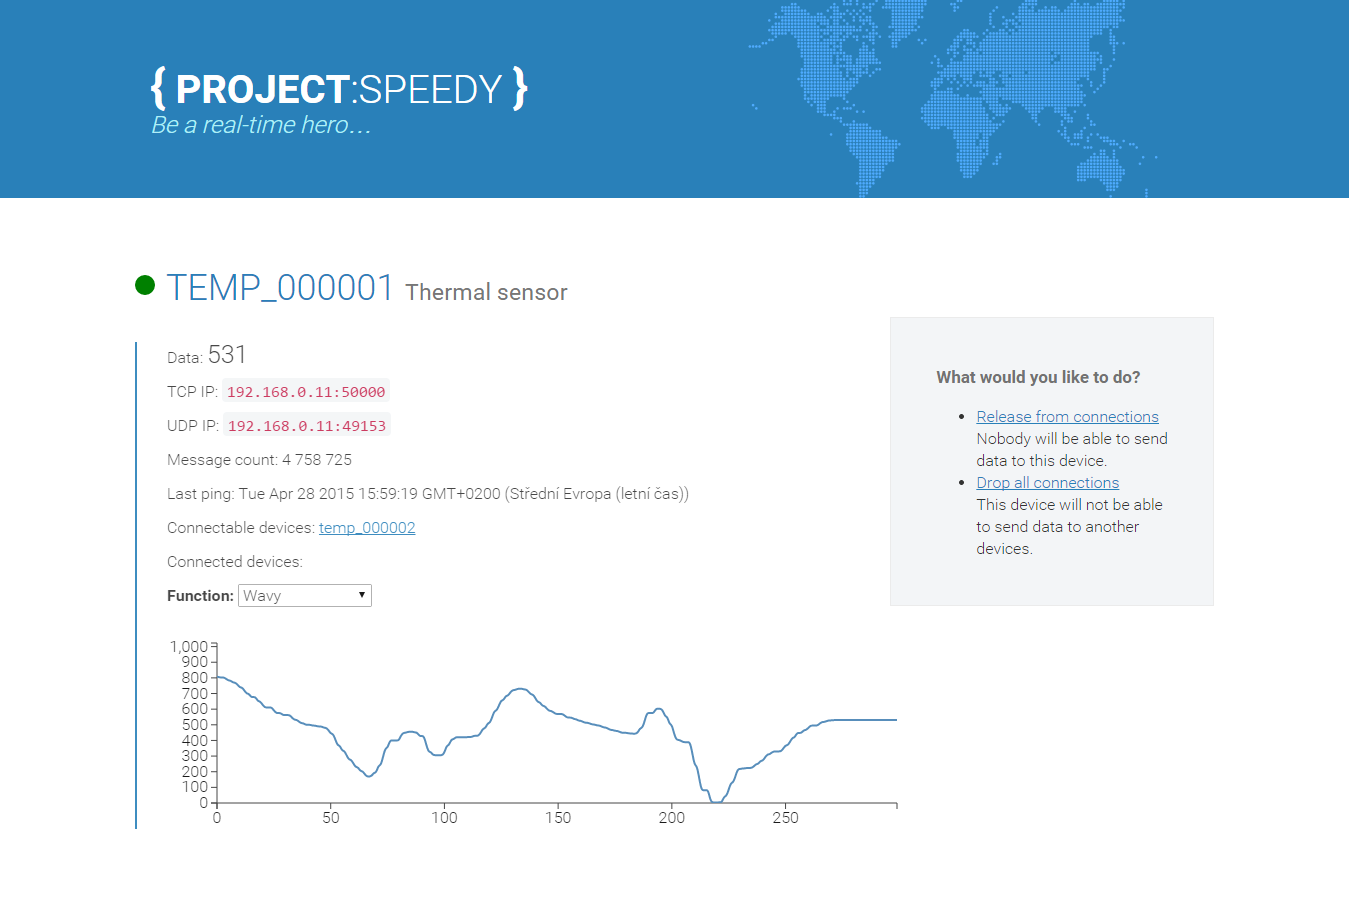
\includegraphics[width=\textwidth]{img/speedy2.png}}
	\caption{Detailní pohled na připojené zařízení}
	\label{fig:speedy2}
\end{figure}

\chapter{Rozšíření stávajícího řešení}
Stávající řešení je plně funkční a splňuje veškeré požadavky v zadání. Jedná se však pouze o základ na kterém lze stavět systém, který by bylo možné použít v reálných budovách. Prvně je totiž zapotřebí tuto síť zabezpečit. To se týká zejména okamžiku, kdy by síť začala komunikovat přes WiFi (nebo jinou bezdrátovou technologii), ale platí to stejně i pro metalické vedení. Nesmí být možné, aby mohl kdokoliv ovlivňovat chování sítě, pokud k tomu není oprávněn.

Dalším důležitým prvkem je implementace IPv6. V současné chvíli je totiž nepsaným předpokladem, že budou koncentrátory připojeny v privátní síti a využívají IPv4. Pokud by však měla síť fungovat i na veřejné síti, vzroste počet potřebných IP adres a již v tuto chvíli je jich nedostatek. Oproti tomu je IPv6 adres je $2^{128}$ \cite{ripe}, což je více než dostatek. V tomto projektu je použit LwIP stack, který IPv6 podporuje. Tato vlastnost není implementována, protože není potřeba. Pokud by se však projekt rozrostl do větších rozměrů, bylo by jej vhodné směřovat do stavu tzv. \uv{fog computingu}. To znamená, že se z původně převážně centralizovaného systému začne stávat silně distribuovaný a původně centralizovaná část sítě bude sloužit pouze pro analýzy a statistiky. Veškeré zpracování dat se bude odehrávat na krajích sítě. Tím se vyřeší například problém s latencí. Zde by již bylo krátkozraké uvažovat překlad IP adres v rámci intranetové sítě, protože jednotlivými koncovými členy sítě mohou být jakákoliv připojitelná zařízení, tedy například automobily, mobilní senzory atd. Překlad IP adres je tedy jednou z možností, ale otázku je, jestli to při tak velkém počtu adres má smysl.

Vzhledem k tomu, že je v současné chvíli celá síť závislá na centrálním serveru, nelze následující požadavek jednoduše implementovat. Bylo by však vhodné, aby se server začal postupně přesouvat na samotné koncentrátory, až by jej vůbec nebylo potřeba. To by znamenalo server úplně horizontálně rozškálovat, což v současnou chvíli není možné. Jednak proto, že by se to z hlediska Node.js nedělalo dobře, jednak také proto, že koncentrátory mají poměrně malý výkon. Malý výkon v tom smyslu, že pro rozumné spuštění Node.js, nebo konkurenčního io.js je nutné Linuxové prostředí. Nicméně reálně fungující projekt využívající OpenWrt Linux \cite{openwrt} s io.js je například Tessel 2 (Cortex\texttrademark-M3 CPU - 180 MHz) \cite{tessel}. Tento krok by přiblížil celý projekt k naprosto autonomní síti, kde by se velmi jednoduše řešil například výpadek jednoho z koncentrátorů. Přestala by totiž fungovat pouze malá část sítě. Navíc by bylo možné částečně se zbavit metalických vodičů a vytvářet tzv. mesh sítě, což by ostatně bylo žádoucí. Každý koncentrátor by se mohl bez větší námahy připojit na všechny koncentrátory, které jsou poblíž.

%TODO opravit následující tvrzení vit připomínky p. Krista

Dále je zajímavou myšlenkou implementovat real-time přenos i na komunikaci mezi koncentrátory a serverem např. Ethernet Powerlink. Zde je však otázka, jestli je tato implementace žádoucí, protože real-time přenos v tomto slova smyslu je právě časově vázaný a svým charakterem tak zpomaluje (i když zpřesňuje) přenos dat. V současné chvíli také není implementováno přijímání adres z DHCP serveru, kvůli jednoduchosti. Na funkcionalitě se nic nemění, je však možné pohodlně vyvíjet, bez nutnosti dalšího prvku v síti.

V neposlední řadě bude také nutné vybavit síť velkým počtem růz\-no\-ro\-dých prvků jako jsou různé vypínače, snímače a akční členy, protože dobrou síť dělá mimo jiného také počet možností, které lze se sítí dělat.